\section{Introduction}

This work serves as a replication study of Levitan et al. (2014), where depolarization block is studied in two simplified models (3-dimensional and 2-dimensional) which are proposed reductions of a more complex 5-dimensional model. In vitro, depolarization block has been shown to limit the maximum firing rate of dopaminergic (DA) neurons \supercite{Richards1997}, and is caused by a sustained, large amplitude membrane current \supercite{Bianchi2012}. The authors’ previous modelling work revealed that a failure to recover from sodium channel inactivation is one way to enter into depolarization block, whereby the availability of sodium channels limits the maximum firing rate of DA cells \supercite{Levitan2014}. Additionally, a slow inactivation ($h_{s}$) component of sodium channel had been previously hypothesized \supercite{Ding2011}. Elaborating on this hypothesis, Levitan et al. (2014) developed a simplified 2D (excluding $h_{s}$), and 3D (including $h_{s}$) model to analyze the role of a slow inactivating component. Both proposed simplified models successfully reproduced the sodium current measured in DA neurons which had been previously described \supercite{Seutin2010}, allowing the authors to faithfully investigate the mechanism of depolarization block. We replicated Figures 1–4 and 6, and in few cases found very minor quantitative differences, as well as two major differences in the results of figure 1c and figure 6.

\section{Methods}

The methods section should explain how you replicated the original results:

This replication was produced using the model described by Levitan et al. (2014), and personal communication with the authors. While the original study computed all simulations, bifurcation diagrams, and nullclines using XPPAUT, our replication was performed using Python (x.y.z); for full package specifications including version numbers, please see the included requirements.txt. The model description was taken directly from page 1 and 2 of the original paper. Additionally, the model gating variables and the model reductions were taken from Table 1 and page 3 respectively. It should also be noted that in order to get the same result shown in figure 1c we changed the time constant equation for the activation of sodium current ($\tau_{n}$) for all simulations as follows: 
 
\begin{center}
	$$\tau_{n^{original}} = 1 + 19 e^{- (\frac{{\ln[1 - 0.05 (v+40)]}}{0.05})^{2}/300}$$
	$$\tau_{n^{modified}} = 1 + 19 e^{- (\frac{{\ln[1 - 0.05 (v+60)]}}{0.05})^{2}/300}$$
\end{center}

As previously mentioned, some further discrepancies were found and will be noted and elaborated on in the discussion section. 


\section{Results}

All figures, with the exception of figure 5 (experimental data), were successfully replicated. Figures 1 and 6 had minor and major discrepancies respectively, which will be addressed accordingly.\\  
In figure 1, the authors show the reliability of their reduced 2/3D models. In figure 1A the authors plotted the peak currents of the models with $h_{s}$ and without $h_{s}$ against experimental data from Seutin and Engel (2010) successfully showing that they had not compromised the original sodium current description.  Our replication (Figure 1A) shows seemingly identical results for the models with and without $h_{s}$. Next, Figure 1B displayed the effect of slow inactivation of sodium current when depolarizing current steps were repeatedly applied. When replicated in Figure 1B, we found that the results were “backwards”. This discrepancy will be discussed later. As part of reducing the 5D model, potassium current ($n$) was modified to a be a function of fast inactivation of sodium current ($f(h)$). This was shown in Figure 1C whereby $f(h)$ and $n$ were plotted against $h$. In order to successfully replicate figure 1C, the time constant $\tau_n$ required modification as shown in the methods section. Figures 1 D1 and 1 D2 compared the 5-D model to the 3-D model respectively. This was well reproduced in our implementation.\\ 

\begin{figure}
	\centering
	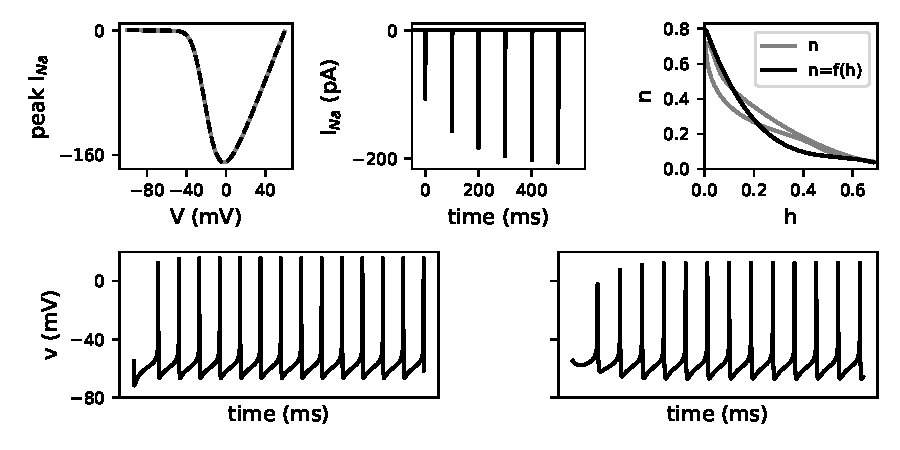
\includegraphics[scale=0.7]{../figures/figure_1.pdf}
	\caption{Replication of model development and reduction. A: Peak sodium voltage-clamp currents with and without $h_{s}$ are identical. B: Slow inactivation of the sodium current with repeated 3-ms depolarizing pulses to 0 mV applied at 100-ms intervals from a holding potential of -70 mV. C: The activation of potassium current ($n$) and the modified potassium current ($f(h)$) plotted against the fast activation of sodium current ($h$). D1: The 5-D model with an applied current of 0 $\mu$A/cm\textsuperscript{2}. D2: The reduced 3-D model with an applied current of 0 $\mu$A/cm\textsuperscript{2}}
	\label{fig:1}
\end{figure}

Figure 2 analyzed the entry into depolarization with the 2D model (without $h_s$). Figure 2A demonstrated that applying a current step caused a “ringing” just before entry into depolarization block (stabilized at -19 mV). This same “ringing” was observed in our replication (Figure 2 A), however it was less prominent and was significantly shorter. Figures 2 B1 and B2 were a nullcline analysis of $h$ with an applied current of 0 $\mu$A/cm\textsuperscript{2} and 3.5 $\mu$A/cm\textsuperscript{2} respectively. Our replication of both showed identical results.\\ 

\begin{figure}
	\centering
	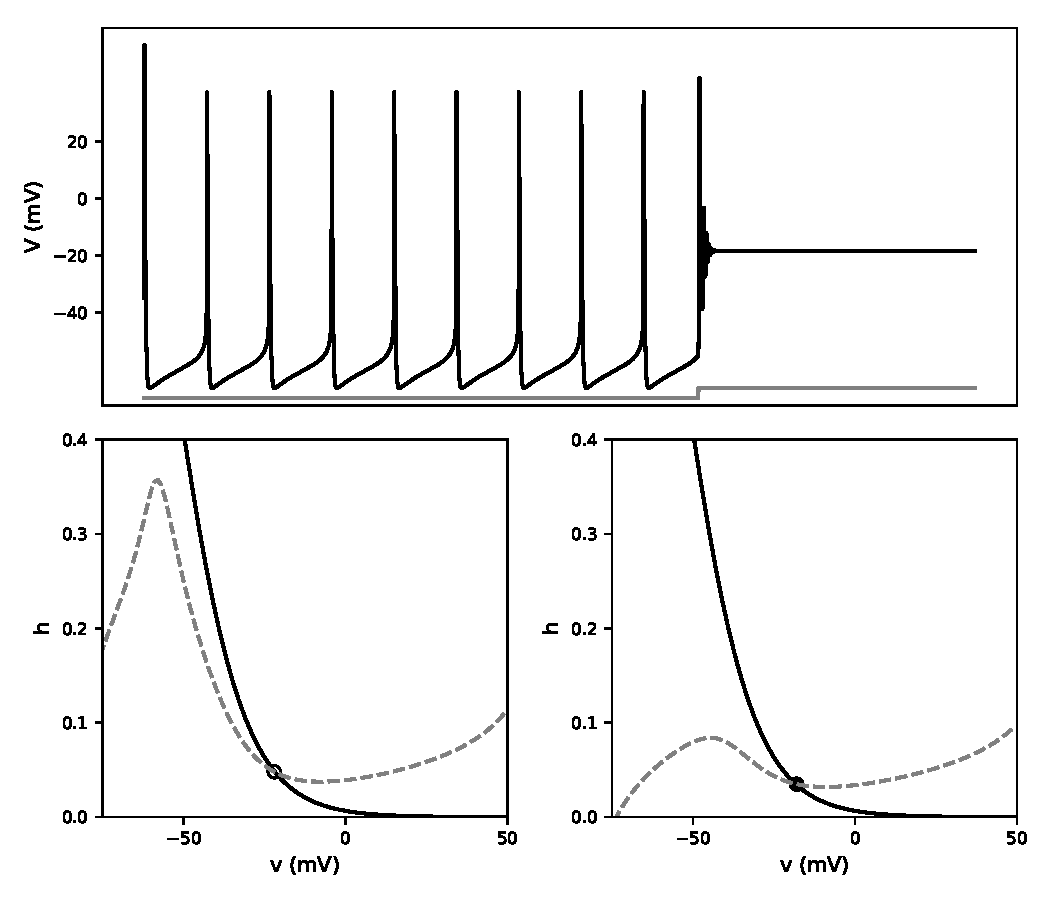
\includegraphics[scale=0.7]{../figures/figure_2.pdf}
	\caption{Entry into depolarization block using the 2-D model. A: A 3.5 $\mu$A/cm\textsuperscript{2} current step applied from 0 $\mu$A/cm\textsuperscript{2} causing entry into depolarization block. B1: The membrane potential nullcline (dashed line) and the sodium channel inactivation nullcline (solid line) intercept at an unstable fixed point (open circle) when the applied current is 0 $\mu$A/cm\textsuperscript{2}. B2: The membrane potential nullcline and the sodium channel inactivation nullcline intersect at at stable fixed point with an applied current at 3.5 $\mu$A/cm\textsuperscript{2}.}
	\label{fig:2}
\end{figure}

Levitan et al. (2014) then analyzed the entry into depolarization block with the 3-D model. Figure 3A1 plotted membrane current of the 3-D model followed by an applied current causing depolarization block. They demonstrate that slow inactivation of sodium current provides a mechanism for spike frequency adaptation as opposed to the “ringing” seen with the 2-D model. This was well reproduced in Figure 3 A1. In Figure 3A2 the authors investigated the contribution of $h_s$ to $h_{total}$ ($h_{total}= h_{s} \times h$) with the same applied current seen in Figure 3A1. This was also well reproduced in Figure 3 A2. \\

\begin{figure}
	\centering
	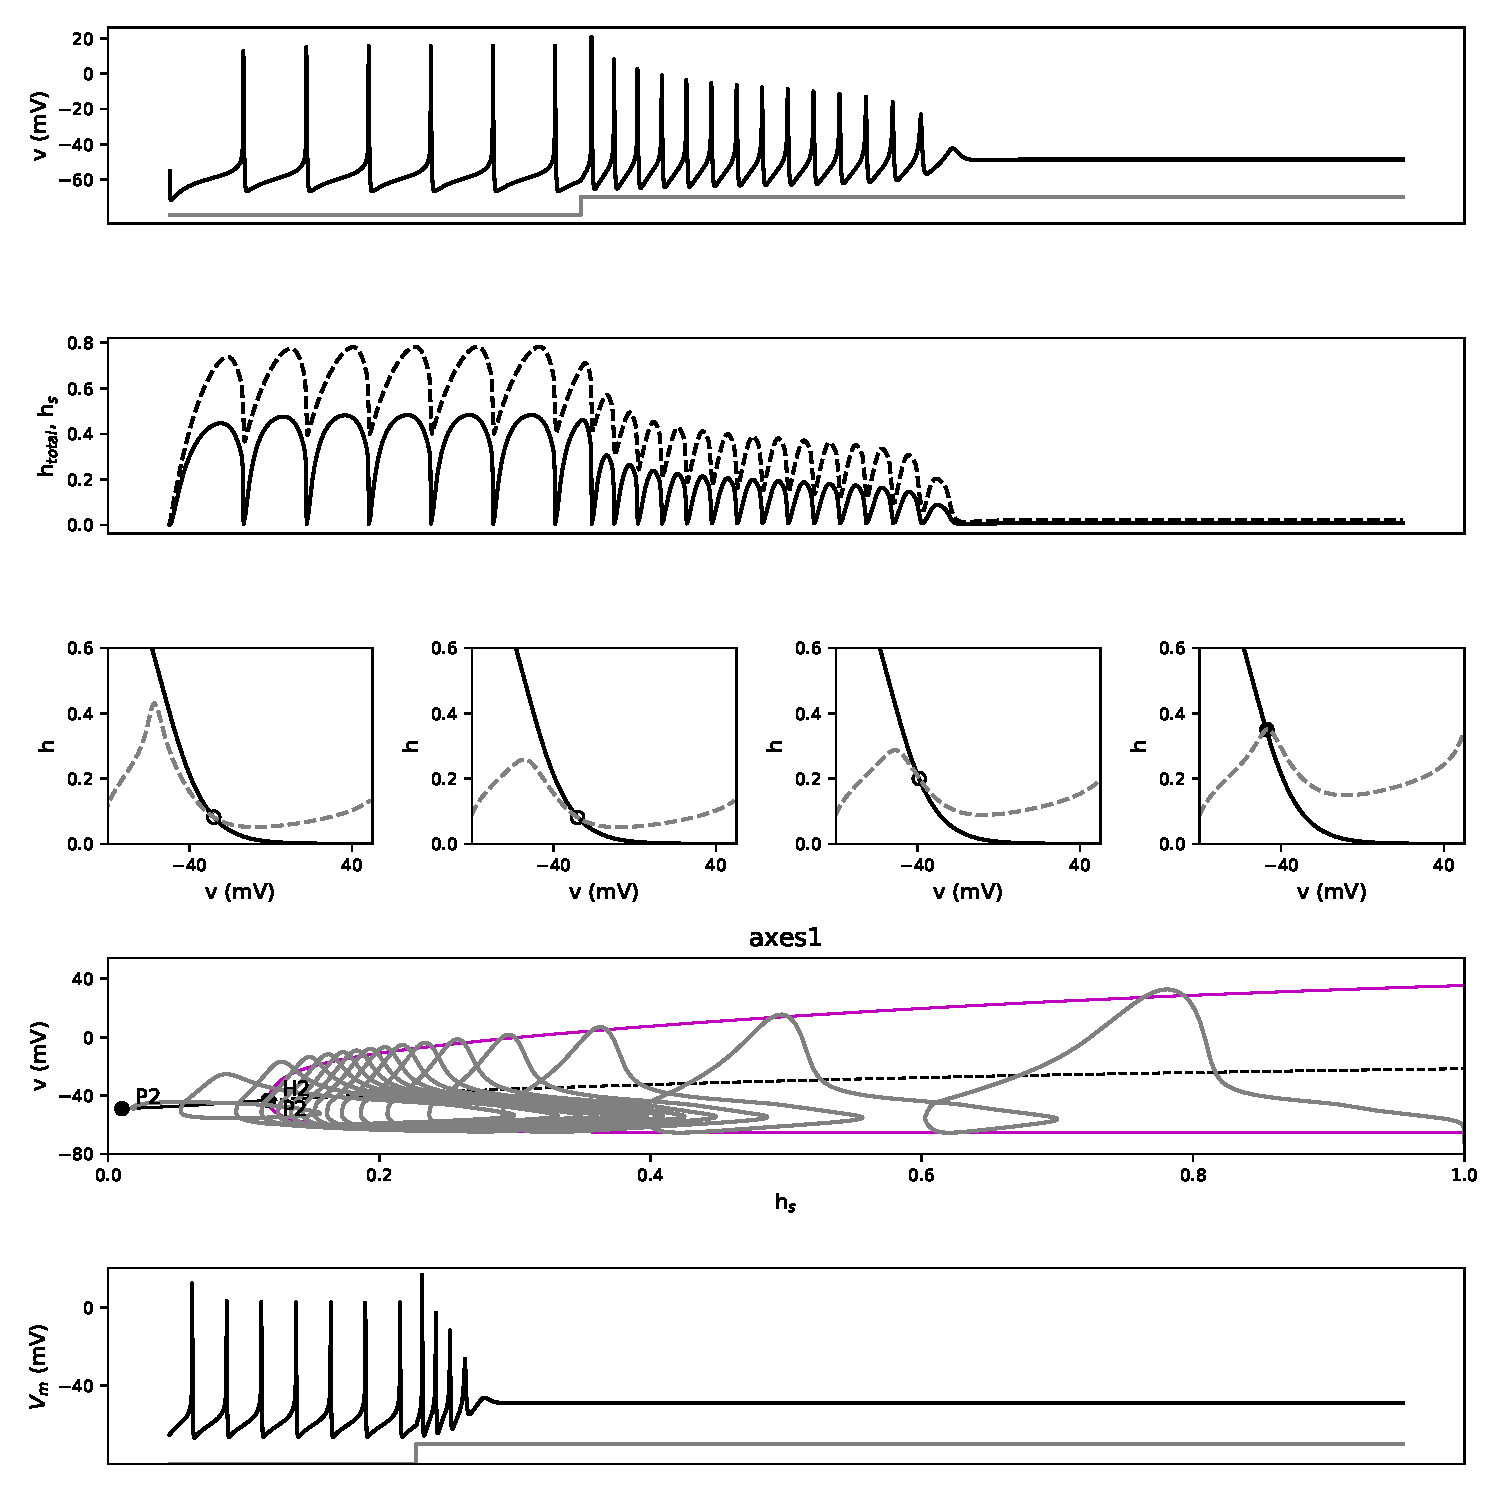
\includegraphics[scale=0.7]{../figures/figure_3.pdf}
	\caption{Entry into depolarization block using the 3-D model. A1: Membrane current with an applied current of 0.16 $\mu$A/cm\textsuperscript{2} from 0 $\mu$A/cm\textsuperscript{2} causing entry into depolarization block. A2: Contribution of $h_s$ (dashed line) to $h_{total}$ (solid line; $h_{total}= h_{s} \times h$) with an applied current of 0.16 $\mu$A/cm\textsuperscript{2} from 0 $\mu$A/cm\textsuperscript{2} causing entry into depolarization block. B1-B4: Membrane potential nullcline (dashed line) and the sodium channel inactivation nullcline (solid line) intersect at different unstable (open circle) and stable (closed circle) fixed points in response to different applied currents and $h_s$ constants. B1: Applied current of 0 $\mu$A/cm\textsuperscript{2} and $h_s$ set to 0.6. B2: Applied current of 0.16 $\mu$A/cm\textsuperscript{2} and $h_s$ set to 0.6. B3: Applied current of 0.16 $\mu$A/cm\textsuperscript{2} and $h_s$ set to 0.2. Applied current of 0.16 $\mu$A/cm\textsuperscript{2} and $h_s$ set to 0.05. C: Bifurcation analysis with $h_s$ as the bifurcation parameter. The trajectory is shown using the grey line, and the supercritical Hopf is denoted by H1. D: The slow inactivation sped up by a factor of 2.}
	\label{fig:3}
\end{figure}

In figures 3B1-B4 the authors also performed a nullcline analysis and outlined the effects of varying the current stimulus and $h_s$ in Figures 3 B1-B4. Our results, shown in Figures 3B1 – B4, correspond to the same outcomes faithfully replicate their results. Similarly, Figures 3C and 3D (corresponding to Levitan et al. 2014 Figures 3C and 3D) were well reproduced. 3C was a bifurcation analysis with $h_s$ as the bifurcation parameter overlaid with the trajectory. 3D showed the results of speeding up slow inactivation of sodium current by a factor of 2.\\ 


\begin{figure}
	\centering
	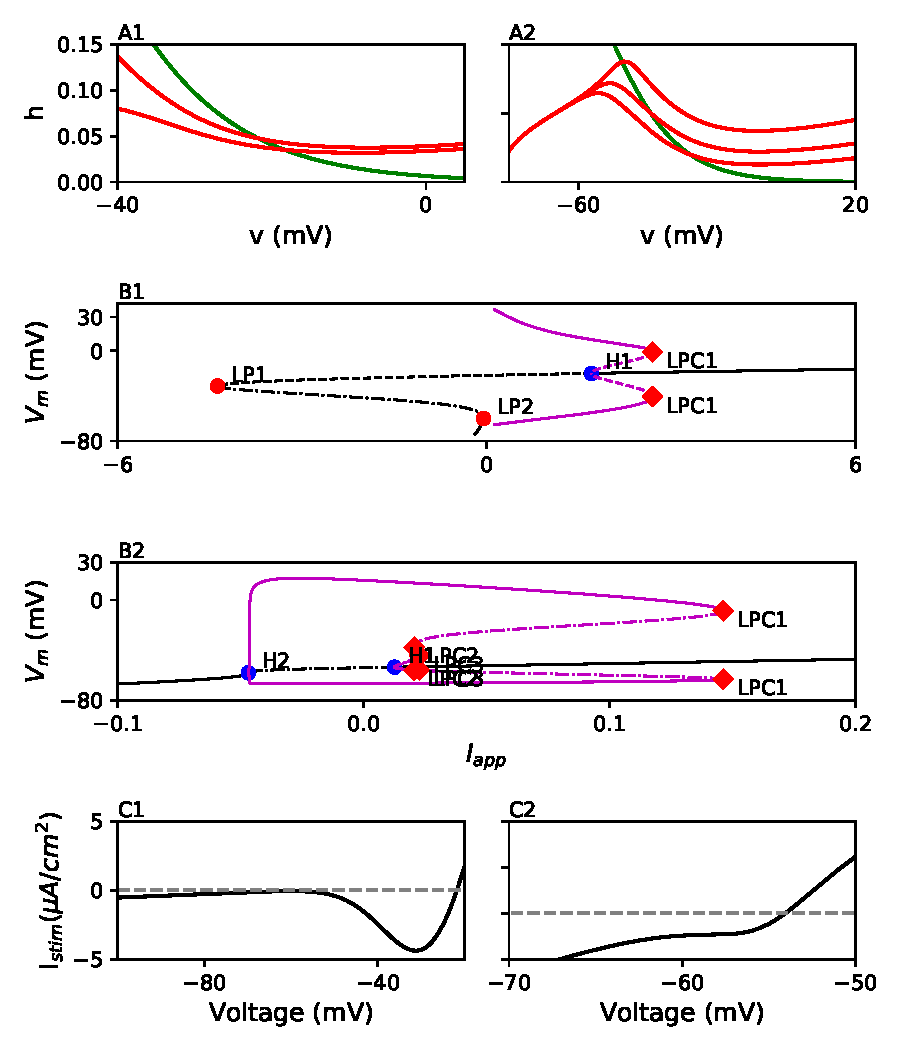
\includegraphics[scale=0.7]{../figures/figure_4.pdf}
	\caption{A1: The voltage nullcline (red) and the $h$ nullcline for the 2-D model as the applied current is increased from 0 to 3.5 $\mu$A/cm\textsuperscript{2} from left to right. A2: The voltage nullcline (red) and the $h$ nullcline for the 3-D model as $h_s$ is decreased from 0.6 to 0.2 to 0.05 from right to left. B1: Bifurcation diagram for the 2-D model showing 3 branches of fixed points to the left of the pacemaking region. B2: Bifurcation diagram for the 3-D model showing the single branch of fixed points. C1: nonmonotonic I-V curve for the 2-D model. C2: monotonic I-V curve for the 3-D model. }
	\label{fig:4}
\end{figure}

Next, the authors used Figure 4 to compare the differences between the 2-D and the 3-D model, thereby analyzing the significance of the slow inactivation of sodium current. In Figure 4 A1 they summarized the nullcline analysis done in Figure 2B, and Figure 4A2 summarized the analysis performed in Figure 3B . Our results (Figure 4A) were well in accordance with what they had produced. To follow that, Levitan et al. (2014) then compared the bifurcation analysis of the 2D model and 3D model in Figures 4B1 and 4B2 respectively. Our replication (Figure 4B) successfully reproduced the stable oscillation, unstable oscillation, unstable fixed points, and fixed points. Lastly, the original works produced current-voltage (I-V) curves, where Figure 4 C1 was the nonmonotonic IV curve (2-D model), and Figure 4C2 was the monotonic IV curve (3-D model). We had successfully reproduced this by clamping the voltage and computing the membrane current across voltage steps, just as Levitan et al. (2014) had done.\\ 


\begin{figure}
	\centering
	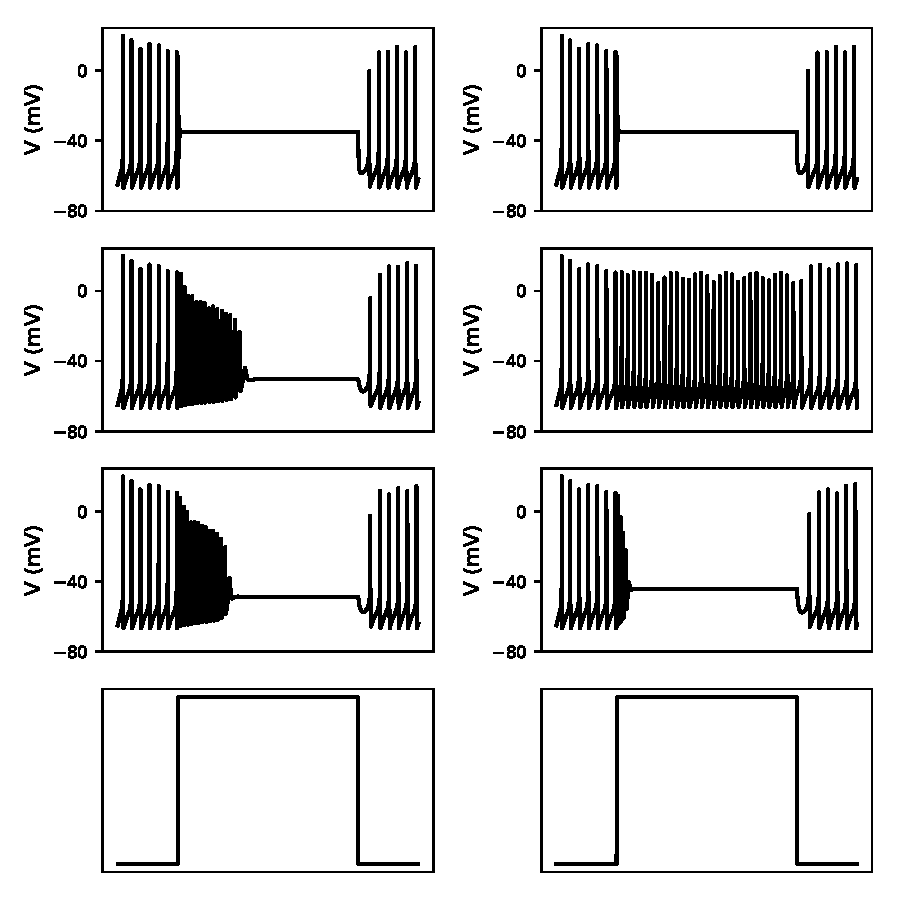
\includegraphics[scale=0.7]{../figures/figure_6.pdf}
	\caption{A1-A3: Square pulses of conductance or current applied to the 3-D model. A1: NMDA conductance pulse of 60 $nS$/cm\textsuperscript{2}. A2: AMPA conductance pulse of 2.3 $nS$/cm\textsuperscript{2}. A3: Applied current pulse of 0.16 $\mu$A/cm\textsuperscript{2}. B1-B3: Comparison of square pulses that were supposed to induce the same level of depolarization as seen in Figure 6 A1-A3 of the original works. B1: NMDA conductance pulse of 60 $nS$/cm\textsuperscript{2}. B2: AMPA conductance pulse of 0.7 $nS$/cm\textsuperscript{2}. B3: Applied current pulse of 0.32 $\mu$A/cm\textsuperscript{2}. }
	\label{fig:6}
\end{figure}

Finally, the authors compared the effects of NMDA and AMPA receptors on entry into depolarization block. As we did not duplicate figure 5, figure 6 corresponds to our figure 5. In Figure 6A1, A2, and A3 they displayed the results coinciding with an applied NMDA conductance, AMPA conductance, or current pulse, respectively. We successfully replicated the current pulse portion of this figure using the 3-D model. However, we found the NMDA and AMPA applied conductance replications to be unsuccessful. After consulting with the authors, we were unable to conclude which parameters had been used and therefore were not able to reproduce these figures. These inconsistencies will be addressed in the discussion section.  

\section{Discussion}

Overall, this implementation replicated the original paper. There were some inconsistencies with the 5-D model (Figure 1) and with the analysis using NMDA and AMPA receptors (Figure 6). More specifically, our replication of Figure 1B was “backwards” where the sodium current decreases towards zero in time, which is opposite in the original implementation. Upon speaking with the authors, they kindly provided us with one of their ODE files for the 3-D model but unfortunately did not have the 5-D model. Hence, we can only speculate that this may have potentially been a graphing error. As previously mentioned, we found some discrepancies with figure 1C which were restored by modifying $\tau_n$  (see Methods). The authors’ ODE file contained a different set of constants for $f(h)$, however, when we ran the model with the new constants, we found negligible qualitative and quantitative differences.  Thus, the modified equation seemed to be the best way to restore the proper model fit given in the original paper. Next, we found that Figure 2A had a shorter and less prominent “ringing” period when entering depolarization block, however the cessation in firing still occurred at -19mV as demonstrated in the original implementation and had identical spikes prior to depolarization block. Lastly, our findings for Figure 6 were dramatically different from that of the initial implementation. With the provided ODE file, it was unclear which conductances were used in the model. Seeing as the bifurcation analysis replicated in figures 3 and 4 were quantitatively identical, we suspect that the reason Figure 6 was unsuccessfully replicated was due to the fact that the original paper used different parameters.

Despite the subtle discrepancies, this model by far demonstrates all the major results using the 2-D and 3-D model were implemented correctly. 

\section{Conclusion}

With the exception of Figure 6, this implementation confidently shows that the original results were correctly implemented. The subtle discrepancies we had found between the original works and our replication were identified and addressed.  
